\appendix

\chapter{Pangolin v1.0, a~conservative 2-D transport model for large scale
parallel calculation}
\label{app:paper}
This paper was accepted by the \gls{GMD} journal.

\input pangolin_paper

\chapter{Supplement}
\section{Proof: number of cells at the poles}
\label{sec:pole_area}
\def\dphi{\Delta\phi}
\def\dlamb{\Delta\lambda}
Here, we demonstrate why the number of cells at the poles for the Pangolin grid
can be approximated by $3$. The latitude spacing is supposed to be "small"
enough and the cells are supposed to be square at the Equator.
We first consider the surface of the band near the Equator, defined by 
$\pi/2 - \dphi \le \phi \le \pi/2$:
\begin{equation*}
  S_{eq} = \int_{0}^{2\pi}\int_{\pi/2}^{\pi/2 - \dphi} r^2 \sin\phi \mathrm{d}\lambda
  \mathrm{d}\phi 
      = 2\pi r^2 \sin \dphi
\end{equation*}
The surface of the band near the North Pole ($0 \le \phi \le \dphi$) is:
\begin{equation*}
  S_{pole} = \int_{0}^{2\pi}\int_{0}^{\dphi} r^2 \sin\phi \mathrm{d}\lambda
  \mathrm{d}\phi 
      = 2\pi r^2 (1-\cos \dphi)
\end{equation*}
The number of cells at the Equator is $2\pi/\dlamb=2\pi/\dphi$ so the area of the cells at
the Equator is:
\begin{equation*}
  \mathcal{A}_{eq}=\frac{S_{eq}}{\frac{2\pi}{\dphi}} = r^2 \dphi \sin \dphi
\end{equation*}
The grid preserves the areas so the number of cells at the pole is:
\begin{equation*}
  n_1 = \Big \lfloor\frac{S_{pole}}{\mathcal{A}_{eq}} \Big \rfloor 
      =\Big \lfloor\frac{2\pi(1-\cos \dphi)}{\dphi \sin
  \dphi } \Big \rfloor 
\end{equation*}
Using small angles approximations, it gives:
\begin{equation*}
  n_1 = \Big \lfloor \frac{2\pi(\frac{\dphi^2}{2})}{\dphi^2} \Big \rfloor = \lfloor \pi
  \rfloor = 3
\end{equation*}

\section{MPI send modes}
\label{app:mpi_send}
The following is taken from
\url{http://www.mcs.anl.gov/research/projects/mpi/sendmode.html}:

% Create a format entry-definition, each with a new paragraph
\def\entry#1#2{\leftskip=0pt \texttt{#1}\par\noindent
\leftskip=1.5cm #2\par\indent}

\entry{MPI\_Send}{will not return until you can use the send buffer. It may or may
not block (it is allowed to buffer, either on the sender or receiver side,
or to wait for the matching receive). 
May buffer; returns immediately and you can use the send buffer. A late
add-on to the MPI specification. Should be used only when absolutely
necessary.}
\entry{MPI\_Ssend}{will not return until matching receive posted.}
\entry{MPI\_Rsend}{may be used \textbf{only} if matching receive already posted. User
responsible for writing a correct program.}
\entry{MPI\_Isend}{
    Nonblocking send. But not necessarily asynchronous. You can
    \textbf{not} reuse the send buffer until either a successful,
    wait/test or you \textbf{know} that the message has been received
    (see \texttt{MPI\_Request\_free}). Note also that while the I refers to
    immediate, there is no performance requirement on \texttt{MPI\_Isend}.
    An immediate send must return to the user without requiring
    a matching receive at the destination. An implementation is
    free to send the data to the destination before returning,
    as long as the send call does not block waiting for a
    matching receive. Different strategies of when to send the
    data offer different performance advantages and
    disadvantages that will depend on the application. 
  }
\entry{MPI\_Ibsend}{buffered nonblocking.}
\entry{MPI\_Issend}{
    Synchronous nonblocking. Note that a Wait/Test will
    complete only when the matching receive is posted. 
}
\entry{MPI\_Irsend}{ As with MPI\_Rsend, but nonblocking.}

\chapter{Design}
\begin{figure}[h]
  \centering
  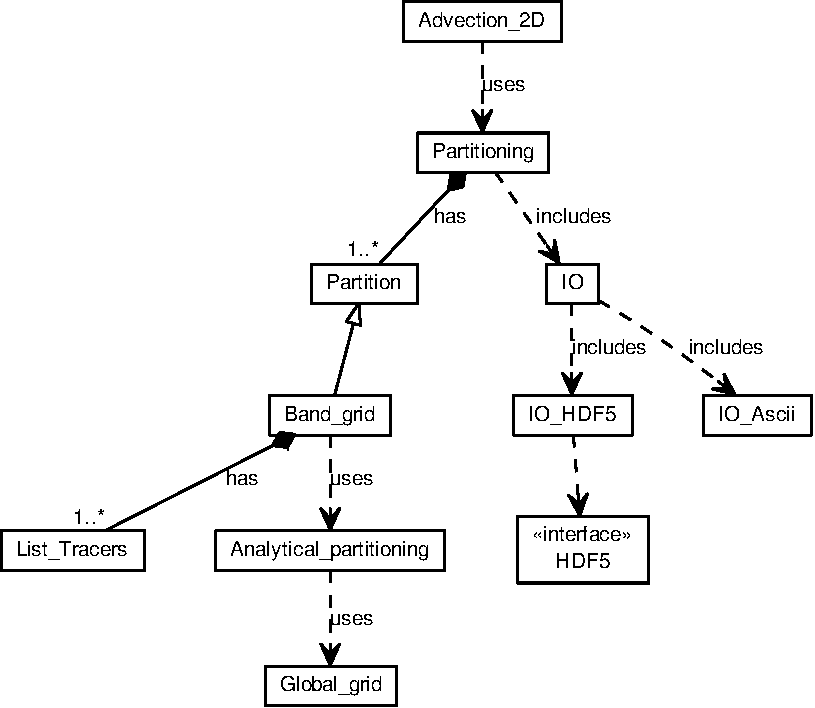
\includegraphics[width=0.9\linewidth]{pangolin_classes.pdf}
  \caption{Classes diagram for Pangolin, with the main classes.}
\end{figure}

\begin{figure}[h]
  \centering
  \includegraphics[width=0.4\linewidth]{flowcharts/pangolin_run.pdf}
  \caption{Flowchart representing a full run in Pangolin. Input winds are
    supposed to be divergence free: there were corrected either during their
    generation (analytical winds) or during interpolation (real winds). As
    temporal interpolation is linear, interpolated winds do not need to be corrected
    either}
  \label{fig:pango_run}
\end{figure}
